\section{Experiments}
\label{cap:experiments}

This section presents an evaluation of the proposed control system. Firstly, simulation results are shown to be subsequently compared real-world experiments. We tested the system in various situations including tracking constant reference, step response and sine trajectory. Another experiments were conducted to verify the disturbance rejection feature. This section also includes observations on drift of the position estimator with an absolute localization system. Finally, the system's performance is compared to the previous work. Most of the experiments are captured in the compilation video \url{http://youtu.be/lPy7w-GUbw4}, which is also located on the enclosed CD. 

\subsection{Simulating MPC}

Figure \ref{fig:simulation_step_no_governor} shows the step response of the system, simulated without the input governor. The proaction can be seen before the step in the reference trajectory, which is enabled due to the predictive nature of the controller. 

\begin{figure}[H]
\centering
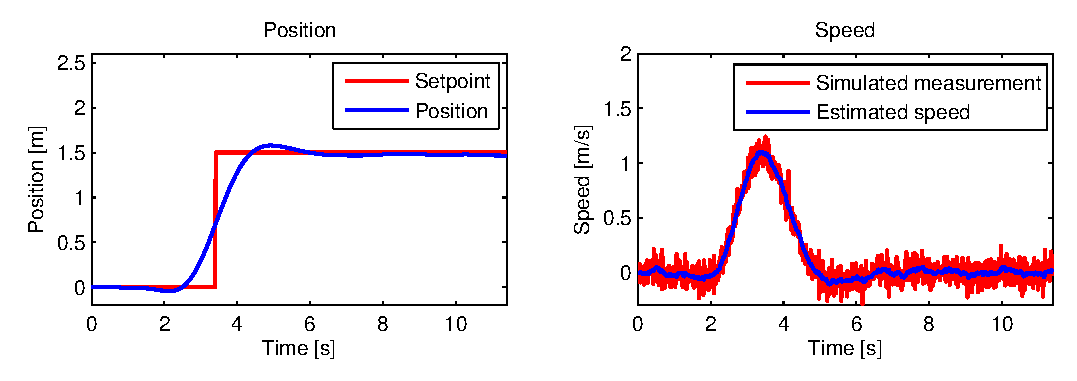
\includegraphics[width=0.99\textwidth]{fig/simulation1_step_no_governor.eps}
\caption{Simulating position step response without the input governor (forward motion).}
\label{fig:simulation_step_no_governor}
\end{figure}

\begin{figure}[H]
\centering
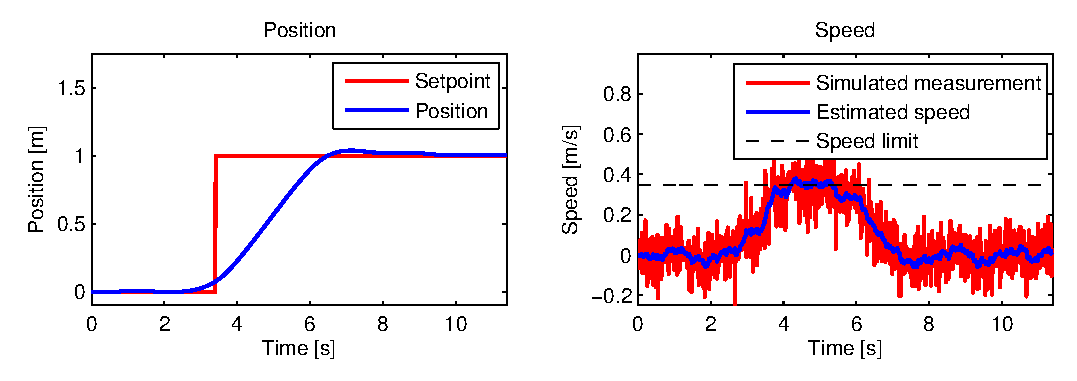
\includegraphics[width=0.99\textwidth]{fig/simulation2_step_governor.eps}
\caption{Simulating position step response with the input governor (forward motion).}
\label{fig:simulation_step_governor}
\end{figure}

Since the desired \emph{unit step} trajectory is not feasible, it should be firstly transformed using the input governor. In our case, we limit the UAV's speed to $0.35\jed{ms^{-1}}$ (which is due to maximum speed that the \emph{px4flow} sensor can measure reliably). Figure \ref{fig:simulation_step_governor} shows the simulation of step response with the input governor. See that the speed lies roughly under the limit. Figure \ref{fig:simulation_sine} shows the simulation of UAV tracking sine trajectory. Prior work \citep{baca2013, endrych2014} and related work \citep{bangura2014realtimempc} demonstrated that tracking such trajectory is difficult without a notable lag. Our simulation shows that MPC with long enough prediction horizon achieves better results. See section \ref{cap:dynamic_trajectory_tracking} for experimental validation of sine trajectory.

\begin{figure}[H]
\centering
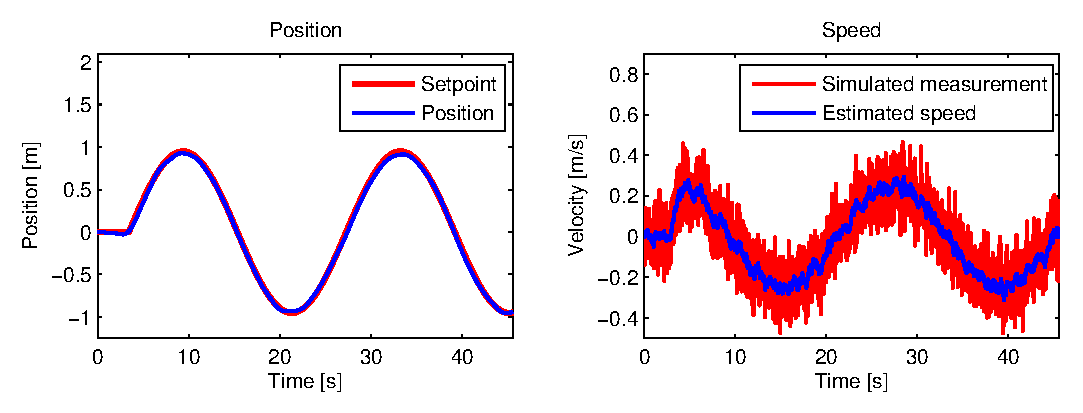
\includegraphics[width=0.99\textwidth]{fig/simulation3_sine.eps}
\caption{Simulating tracking of feasible sine trajectory (forward motion).}
\label{fig:simulation_sine}
\end{figure}

The disturbance rejection ability based on the disturbance estimation is one of key points of the system. It should be able to deal with constant disturbances (cause by bad trimming, offset in \emph{KK2} stabilization) as well as momentary disturbances (possibly caused by wind). Although simulations showed that the disturbance estimation can be tuned arbitrarily to match a desired settling time of the estimate, in practice, there is a limit (see discussion in section \ref{cap:persistant_wind_disturbances_experiment}). Figure \ref{fig:simulation_disturbance_rejection} shows a simulation of disturbance rejection with parameters tuned using the real UAV.

\begin{figure}[H]
\centering
\includegraphics[width=0.99\textwidth]{fig/simulation4_disturbance_rejection.eps}
\caption{Simulation of disturbance rejection (forward motion).}
\label{fig:simulation_disturbance_rejection}
\end{figure}

\subsection{Tracking constant setpoint}
\label{cap:tracking_constant_trajectory}

The first experiment was realized with the aim to test the UAV capability of tracking a constant reference, i.e. hovering above one place. Statistically, we are interested in the standard deviation $\sigma$ and the maximum deviation $\Delta_{max}$. Figure \ref{fig:experiment_constant_trajectory} shows its performance in good light conditions with no wind disturbances. The aircraft was capable of tracking the reference with standard deviation $\sigma = 4.8\jed{cm}$ and maximum deviation $\Delta_{max} = 14.4\jed{cm}$.

\begin{figure}[H]
\centering
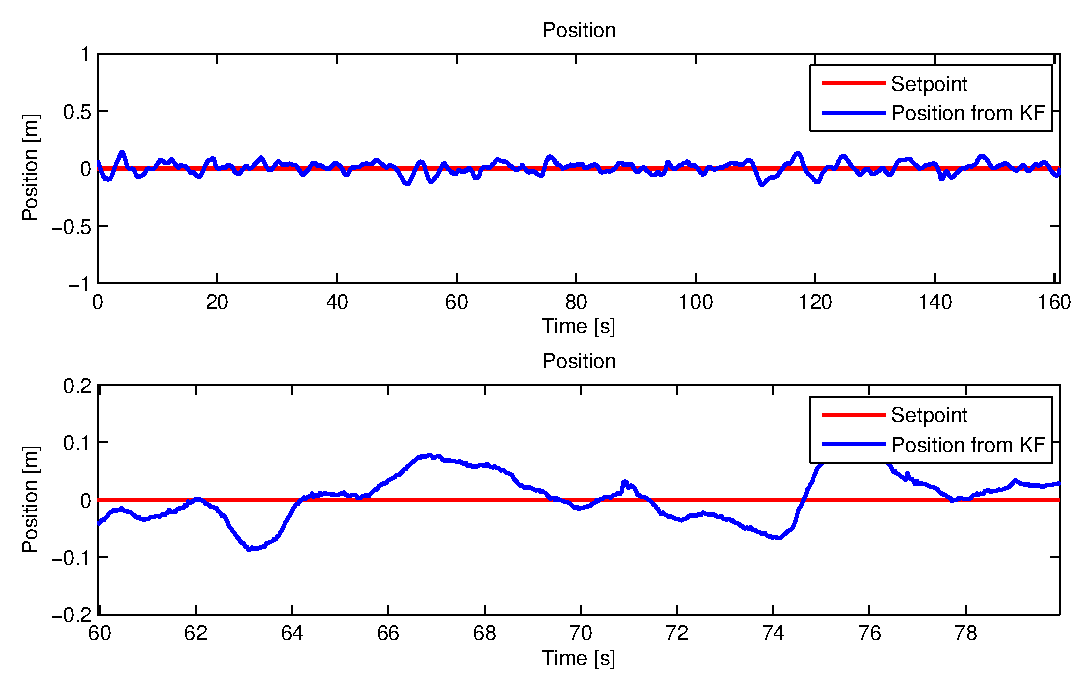
\includegraphics[width=0.99\textwidth]{fig/experiment6_constant_reference.eps}
\caption{Experiment of tracking static trajectory (forward motion).}
\label{fig:experiment_constant_trajectory}
\end{figure}

\subsection{Measuring of estimation drift}

One could ask, what is the relevance of previously presented data, since the position is estimated onboard using only velocity data and the model. The truth is that the position is not absolute and although the controller seems to stay around the setpoint, the absolute position in the space may drift away. In order to measure such drift we implemented the Whycon camera localization system \citep{krajnik14JINT, faigl2013whycon} using calibrated camera was employed. It was used to measure the absolute position of the UAV while conduction a flight. The figure \ref{fig:experiment_drift_constant} shows the position drift during 1 minute flight. The maximum measured deviation was $\approx 10\jed{cm}$. It can be seen, that the estimated position slowly drifts away from the absolute one, and then lately drifts back. Similar effect can be observed in figure \ref{fig:experiment_drift_sine}, where the UAV is tracking a sine trajectory. In general, the drift is larger when the UAV is moving closer to the saturation of the \emph{px4flow} sensor.

\begin{figure}[H]
\centering
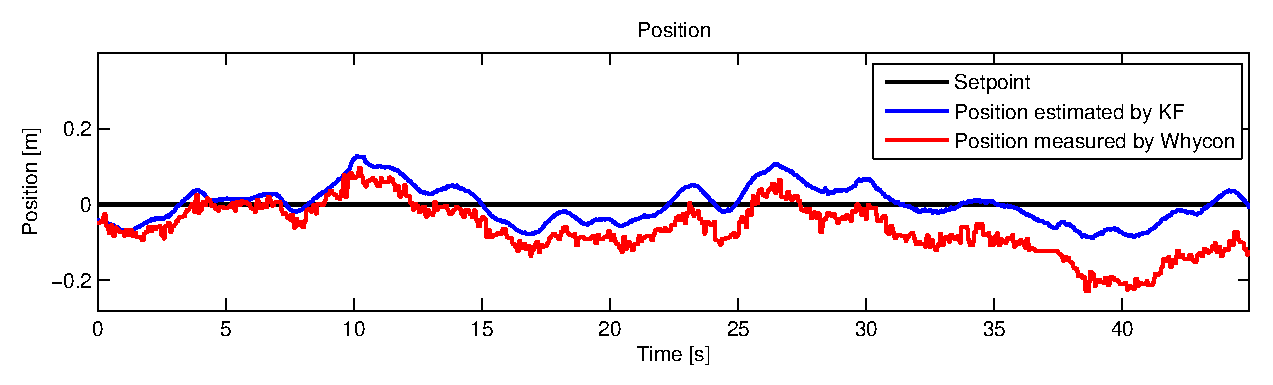
\includegraphics[width=0.99\textwidth]{fig/experiment5_drift_constant.eps}
\caption{Experiment of measuring a position drift (forward motion).}
\label{fig:experiment_drift_constant}
\end{figure}

The signal noise from the \emph{px4flow} sensor is usually larger at higher velocities. At last, there are other conditions that need to be met to eliminate the position drift --- good light conditions and good vibration isolation of the sensor. Otherwise the drift is $\approx 10\jed{cm/min}$ or larger. Our observations correspond with results presented by authors of the system in \citep{honegger2013open}.

\begin{figure}[H]
\centering
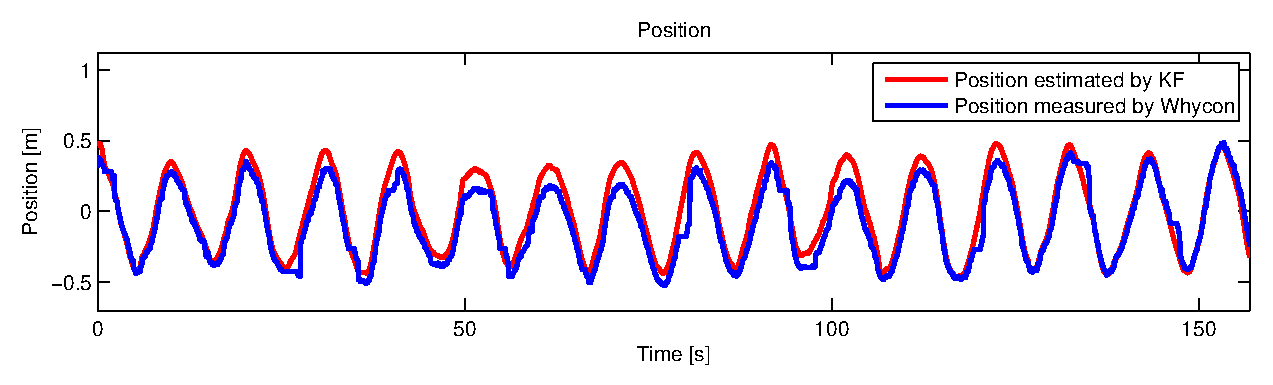
\includegraphics[width=0.99\textwidth]{fig/experiment5_drift_sine.eps}
\caption{Experiment conducted to measure a position drift while tracking a sine trajectory (forward motion).}
\label{fig:experiment_drift_sine}
\end{figure}

\subsection{Tracking dynamic trajectory}
\label{cap:dynamic_trajectory_tracking}

Another experiment tested the system capability of tracking dynamic trajectories. In the first experiment, response of the UAV to a \emph{unit step} response was tested. As it can be seen in figure \ref{fig:experiment_step}, the UAV does not overshoot the setpoint, but it rather makes a proaction which is a typical characteristic of the model predictive controller. The speed lies within the set boundaries due to input governor. Figure \ref{fig:experiment_sine_1} shows the performance of the system during tracking a circular trajectory. The trajectory was precomputed with constant speed $0.25\jed{ms^{-1}}$. Figure shows position and speed for both attitude axis. The experiment can bee seen in the compilation video which can be found at \url{http://youtu.be/lPy7w-GUbw4} or in the enclosed CD (\texttt{video1.mp4}). The maximum deviation from the desired trajectory (forward motion) was $\Delta_{max} = 16.3\jed{cm}$ and the standard deviation $\sigma = 4.3\jed{cm}$.

\begin{figure}[h]
\centering
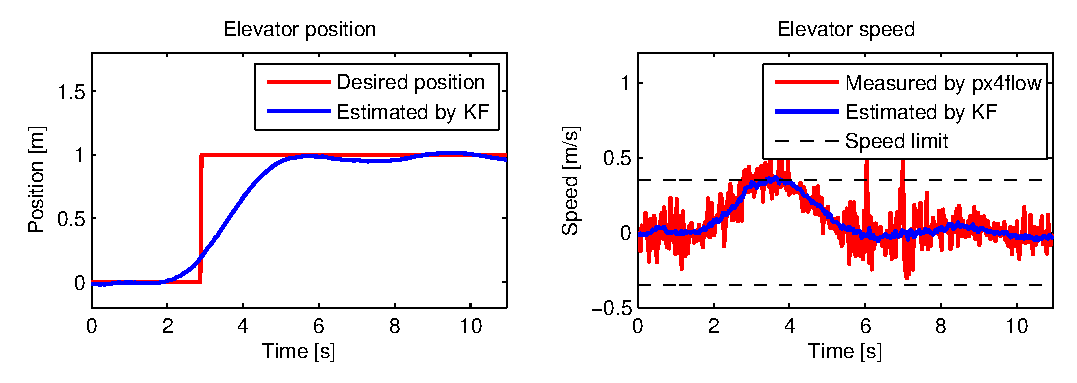
\includegraphics[width=0.99\textwidth]{fig/experiment2_step.eps}
\caption{Experiment of tracking the \emph{unit step} response.}
\label{fig:experiment_step}
\end{figure}

\begin{figure}[H]
\centering
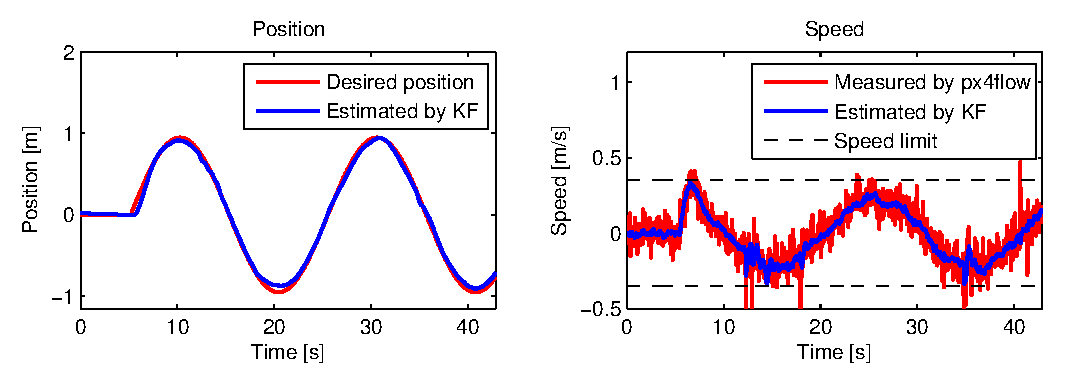
\includegraphics[width=0.99\textwidth]{fig/experiment1_sine.eps}
\caption{Experiment of tracking circular trajectory. Amplitude $0.95\jed{m}$, period $20\jed{s}$, speed $0.25\jed{ms^{-1}}$.}
\label{fig:experiment_sine_1}
\end{figure}

\subsection{Disturbance rejection}

\begin{figure}[b]
\centering
\includegraphics[width=0.75\textwidth]{fig/disturbance.jpg}
\caption{Experimental setup with $40\jed{W}$ fan to test the disturbance rejection feature.}
\label{fig:vetrak1}
\end{figure}

Different set of experiments was conducted to test the disturbance rejection capability. Since we dealt with the real hardware where the dynamical model is only an approximation of the real system, we cannot suppose the same performance during the experiments as it was observer in simulations. The difference was mostly observed during tuning of the disturbance estimator. By decreasing the settling time of the estimated disturbance, the system becomes unstable due to oscillations being induced into the estimate which led to worse performance. We found sufficient parameters that allows to estimate usual disturbances, such as bad trimming or stabilization offset, in order of seconds.
 
\subsubsection{Persistent wind disturbances}
\label{cap:persistant_wind_disturbances_experiment}

The UAV was tested for its capability to reject wind disturbances by using a $40\jed{W}$ fan pointed to the UAV (see figure \ref{fig:vetrak1}). To put it into context, it is the same power as one of UAV motors. The figure \ref{fig:experiment_steady_wind} shows the forward motion of the aircraft. The grey area indicates when the fan was turned on. The estimated disturbance settled in $\approx 10\jed{s}$ which allowed the UAV to eliminate the resulting \emph{steady state} error. Notice the non-zero disturbance when the fan is turned off, which is caused by already mentioned trimming and stabilization offset.

\begin{figure}[h]
\centering
	\begin{tikzpicture}
		\node[anchor=south west,inner sep=0] (a) at (0,0) {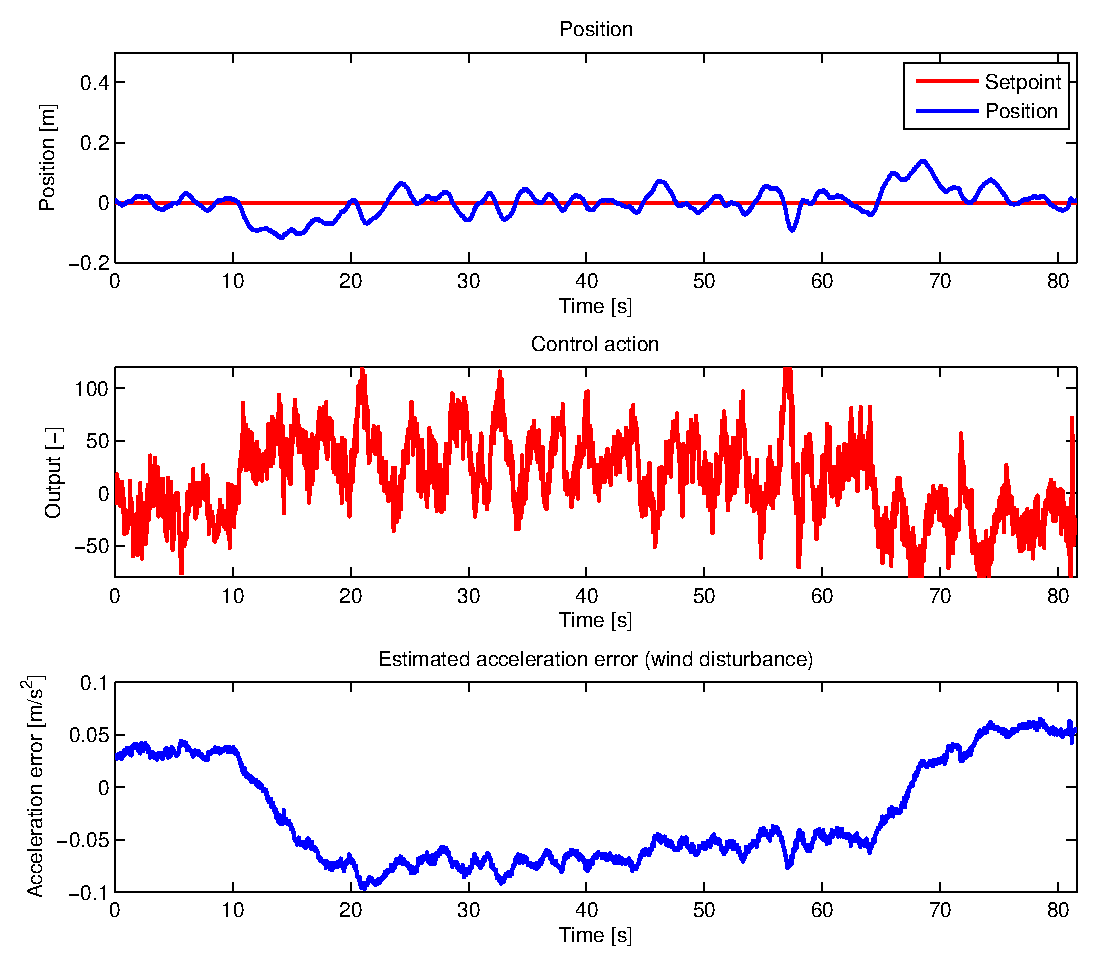
\includegraphics[width=\textwidth]{fig/experiment3_steady_disturbance.eps}};
		\begin{scope}[x={(a.south east)},y={(a.north west)}]

		%\draw[help lines,xstep=.1,ystep=.1] (0,0) grid (1,1);	
		
%        \draw[white,ultra thick,rounded corners] (0.55,0.50) rectangle (0.7,0.7);
%        \draw (0.58,0.655) node [text=white] {\textbf{1}};
        

		%\draw[-latex] (0.2,0.9) -- (0.2,0.81);    
		%\node[] at (0.25,0.92) {Disturbance started};    
		
		%\draw[-latex] (0.75,0.9) -- (0.795,0.81);    
		%\node[] at (0.65,0.92) {Disturbance went off};  
		
		\draw[fill=gray, opacity=0.2] (0.182,0.740) rectangle (0.754,0.961);  
	
		\draw[fill=gray, opacity=0.2] (0.182,0.401) rectangle (0.754,0.624);  
		
		\draw[fill=gray, opacity=0.2] (0.182,0.064) rectangle (0.754,0.286);  
        
    \end{scope}
	\end{tikzpicture}
\caption{Experiment of tracking constant setpoint while being under the influence of wind.}
\label{fig:experiment_steady_wind}
\end{figure}

\subsubsection{Momentary disturbances}
\label{cap:momentary_disturbances}

Following experiment, shown in the compilation video, aimed to test the system's capability of rejecting momentary disturbances. Figure \ref{fig:experiment_momentary_disturbances} shows a forward motion of the UAV, which is repeatedly dragged by hand. These disturbances were short and sudden, and their estimate has relatively short raise time, comparing to those in the previous experiment. Gray areas denote the moments when the UAV was dragged away. One can spot overshoots in the position signal. They can be explained by the remaining disturbance in the estimate. The controller accounted for a disturbance, that was not actually effecting the UAV at the moment (due to the settling time of the estimate). See Appendix \ref{ape:experiments} for additional data from experiments with disturbances.

\begin{figure}[h]
\centering
	\begin{tikzpicture}
		\node[anchor=south west,inner sep=0] (a) at (0,0) {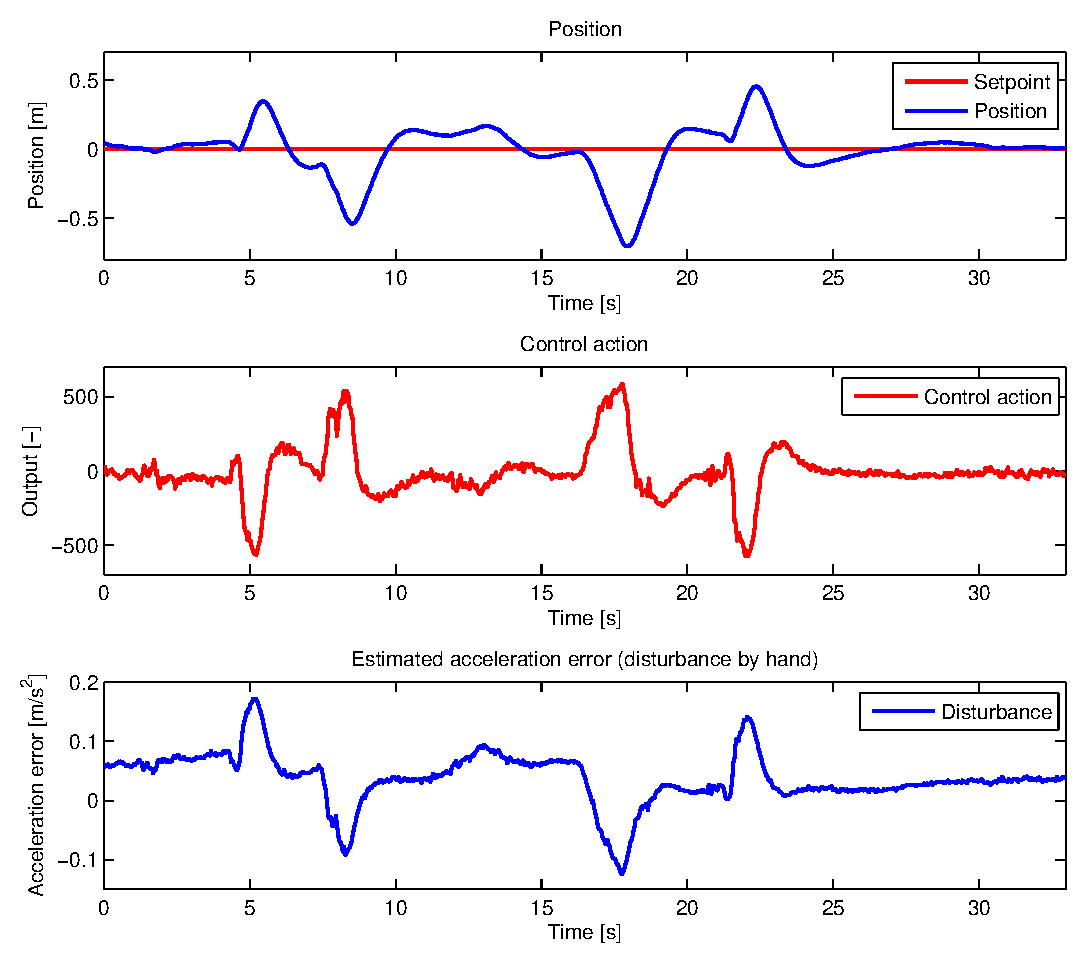
\includegraphics[width=\textwidth]{fig/experiment4_sudden_disturbances.eps}};
		\begin{scope}[x={(a.south east)},y={(a.north west)}]

%		\draw[help lines,xstep=.1,ystep=.1] (0,0) grid (1,1);	
		
%        \draw[white,ultra thick,rounded corners] (0.55,0.50) rectangle (0.7,0.7);
%        \draw (0.58,0.655) node [text=white] {\textbf{1}};

		\draw[fill=gray, opacity=0.2] (0.204,0.7395) rectangle (0.225,0.961);  
		\draw[fill=gray, opacity=0.2] (0.287,0.7395) rectangle (0.310,0.961);  
		\draw[fill=gray, opacity=0.2] (0.41,0.7395) rectangle (0.440,0.961);  
		\draw[fill=gray, opacity=0.2] (0.532,0.7395) rectangle (0.571,0.961);  
		\draw[fill=gray, opacity=0.2] (0.668,0.7395) rectangle (0.69,0.961); 
		
		\draw[fill=gray, opacity=0.2] (0.204,0.402) rectangle (0.225,0.623);  
		\draw[fill=gray, opacity=0.2] (0.287,0.402) rectangle (0.310,0.623);  
		\draw[fill=gray, opacity=0.2] (0.41,0.402) rectangle (0.440,0.623);  
		\draw[fill=gray, opacity=0.2] (0.532,0.402) rectangle (0.571,0.623);  
		\draw[fill=gray, opacity=0.2] (0.668,0.402) rectangle (0.69,0.623); 
		
		\draw[fill=gray, opacity=0.2] (0.204,0.0645) rectangle (0.225,0.2855);  
		\draw[fill=gray, opacity=0.2] (0.287,0.0645) rectangle (0.310,0.2855);  
		\draw[fill=gray, opacity=0.2] (0.41,0.0645) rectangle (0.440,0.2855);  
		\draw[fill=gray, opacity=0.2] (0.532,0.0645) rectangle (0.571,0.2855);  
		\draw[fill=gray, opacity=0.2] (0.668,0.0645) rectangle (0.69,0.2855); 
        
    \end{scope}
	\end{tikzpicture}
\caption{Experiment of tracking constant setpoint while being under the influence of momentary disturbances. The UAV was dragged by hand which is indicated by the gray areas.}
\label{fig:experiment_momentary_disturbances}
\end{figure}

\vfill

\subsection{Outdoor experiment --- longer trajectory}

The last experiment was conducted to present the UAV capability of autonomous operation not only in indoor (laboratory) conditions, but also in a general outdoor area. The UAV was supposed to track a precomputed trajectory with 1 minute duration. Figure \ref{fig:experiment_venku_sipky} shows a photo that illustrates the course of the experiment\footnote{The photo was created by stitching multiple images from the video.} while figure \ref{fig:experiment_venku_plot} shows the plot of onboard data including desired and estimated position. The experiment was conducted under the influence of mild and steady breeze. The video from the experiment can be found on url \url{http://youtu.be/iqgL1H_DCmU} or on the CD (\texttt{video2.mp4}).
\begin{figure}[H]
\centering

\begin{subfigure}[b]{0.5\textwidth}
	\centering
\begin{tikzpicture}
		\node[anchor=south west,inner sep=0] (a) at (0,0) {\includegraphics[width=0.9\textwidth]{fig/experiment7_stitch.jpg}};
		\begin{scope}[x={(a.south east)},y={(a.north west)}]

		%\draw[help lines,xstep=.1,ystep=.1] (0,0) grid (1,1);	
		
%        \draw[white,ultra thick,rounded corners] (0.55,0.50) rectangle (0.7,0.7);
%        \draw (0.58,0.655) node [text=white] {\textbf{1}};
        

		\draw[-latex, color=white, ultra thick] (0.22,0.28) -- (0.425,0.6);   
		\draw[-latex, color=white, thick] (0.47,0.68) -- (0.52,0.75);   
		\draw[-latex, color=white, thick] (0.6,0.8) -- (0.74,0.8);   
		\draw[-latex, color=white, thick] (0.75,0.78) -- (0.705,0.755);      
		\draw[-latex, color=white, thick] (0.7,0.74) -- (0.74,0.715);       
		\draw[-latex, color=white, thick] (0.74,0.66) -- (0.6,0.57);       
		\draw[-latex, color=white, very thick] (0.58,0.5) -- (0.75,0.35);          
		\draw[-latex, color=white, ultra thick] (0.7,0.2) arc (70:110:0.6);
		%\node[] at (0.25,0.92) {Disturbance started};    
		
		%\draw[-latex] (0.75,0.9) -- (0.795,0.81);    
		%\node[] at (0.65,0.92) {Disturbance went off};  
        
    \end{scope}
	\end{tikzpicture}
	\caption{image stitched from the video}
	\label{fig:experiment_venku_sipky}
\end{subfigure}%
\begin{subfigure}[b]{0.5\textwidth}
	\centering
	\includegraphics[width=\textwidth]{fig/experiment7_3D.eps}
	\caption{visualization of logged data}
	\label{fig:experiment_venku_plot}
\end{subfigure}

\caption{Experiment with trajectory conducted outdoors. For detailed data see Appendix~\ref{ape:experiments}.}
\label{fig:experiment_venku}
\end{figure}

Most of previously presented situations can be seen in the compilation video. It is accompanied by data logged onboard the UAV, that are rendered in the video (see figure \ref{fig:video1}). The estimated position is also fitted with the estimated force acting on the UAV. The outdoor video is also accompanied with the position plot (figure \ref{fig:video2}).

\begin{figure}[H]
\centering

\begin{subfigure}[b]{0.5\textwidth}
	\centering
	\includegraphics[width=0.9\textwidth]{fig/experiment1_video.jpg}
	\caption{\texttt{video1}: \url{http://youtu.be/lPy7w-GUbw4}}
	\label{fig:video1}
\end{subfigure}%
\begin{subfigure}[b]{0.5\textwidth}
	\centering
	\includegraphics[width=0.9\textwidth]{fig/experiment2_video.jpg}
	\caption{\texttt{video2}: \url{http://youtu.be/iqgL1H_DCmU}}
	\label{fig:video2}
\end{subfigure}

\caption{Two videos with onboard data rendered --- a) compilation video, b) long trajectory video.}
\label{fig:videos}
\end{figure}

\subsection{Performance and comparison}

Results presented in this section were gathered from three experiments --- tracking constant trajectory (section \ref{cap:tracking_constant_trajectory}), tracking circular trajectory (section \ref{cap:dynamic_trajectory_tracking}), and the last experiment of tracking a longer trajectory in outdoor environment (see the previous section). The first two experiments were performed indoor and all of them were conducted under good lighting conditions. Table \ref{tab:compparison1} shows the statistical evaluation of trajectory tracking where $\sigma_x$, $\Delta_{x, max}$ and $\sigma_y$, $\Delta_{y, max}$ denote the standard and maximum deviation for the lateral and forward axis respectively, and $l$ indicates the time duration of the experiment. One can see that the performance of the system in the indoor environment is slightly better than in the outdoor environment, but overall the results are better when comparing to the previous work \citep{endrych2014}. Although the performance of tracking constant trajectory is similar, the results of tracking dynamical trajectory are in order of magnitude better in terms of the standard deviation. According to results of thesis \citep{endrych2014} it rarely went under 60\jed{cm}. 

\begin{table}[h]
\centering
\begin{tabular}{lrrrrr}
\hline
 & $\sigma_x$ [cm] & $\Delta_{x, max}$ [cm] & $\sigma_y$ [cm] & $\Delta_{y, max}$ [cm] & $l$ [s]\\
\hline
\textbf{constant trajectory} & 4.0 & 15.1 & 3.3 & 11.8 & 184 \\
\textbf{circular trajectory} & 4.3 & 14.9 & 3.9 & 8.5 & 92\\
\textbf{outdoor experiment} & 8.7 & 23.5 & 7.0 & 21.6 & 55\\
\hline
\end{tabular}
\caption{Performance of the proposed solution.}
\label{tab:compparison1}
\end{table}

The result of the proposed system are similar to results of previously used PID controller, if tracking a constant setpoint. If tracking a dynamical trajectory, the MPC outperforms the PID controller significantly.

\subsection{Summary}

The last section of this thesis demonstrated the performance of the system in practice. The implemented Kalman filter was able to estimate external disturbances, which significantly improved performance of the system during offset-free tracking. The UAV was able to effectively counteract wind disturbances. Moreover, it was able to follow a desired trajectory with precision suitable for use in GPS-denied and indoor environment. Statistically, the results were significantly better than in the previous work. 